
\subsubsection{5.1 Mechanism Gate: Normalized SSD Error Decreases with N (RQ1)}

The mechanism gate passes both criteria with large margin.

\begin{table*}[htbp]
\centering
\resizebox{\dimexpr 2\columnwidth+\columnsep\relax}{!}{%
\begin{tabular}{lllll}
\toprule
N & Measurements (n) & Mean error/N & Std/N & 90th pct/N \\
\midrule
512 & 1,600 & 0.0392 & 0.0071 & 0.0478 \\
1,024 & 160 & 0.0331 & 0.0057 & 0.0383 \\
2,048 & 160 & 0.0235 & 0.0043 & 0.0273 \\
\bottomrule
\end{tabular}
}
\end{table*}

\textbf{Log-log slope $\beta = -0.368$} (threshold $\leq$ 0.5 ✓). \textbf{90th percentile at N = 2048 = 0.027} (threshold $\leq$ 0.3 ✓).

For reference, the corresponding raw Frobenius values (unnormalized) are: mean 20.05 at N = 512, 33.89 at N = 1,024, 48.18 at N = 2,048 --- a raw slope of approximately 0.63, reflecting the expected super-linear scaling of Frobenius norm with matrix dimension. Normalization by N reduces this to the sub-linear regime.

Normalized error decreases by approximately 23\% per doubling of N. No layer among the 32 LLaMA-3.1-8B transformer layers is an outlier: the error distribution shifts downward uniformly as N increases (Figure 2).

The negative slope is stronger than the hypothesis required. The gate was pre-registered to allow sub-linear \textit{growth} (slope $\leq$ 0.5); the observed slope is negative, indicating the SSD approximation becomes proportionally \textit{better} at longer contexts. One plausible explanation is that LLaMA-3.1-8B attention matrices become lower-dimensional (more sparse, more concentrated on fewer positions) at longer N due to head specialization and diluted attention mass, creating a lower-effective-rank approximation target that a fixed-rank SSD captures more efficiently. This explanation is consistent with attention sparsity observations in large transformer models but has not been tested directly in this work.

\begin{figure}[htbp]
\centering
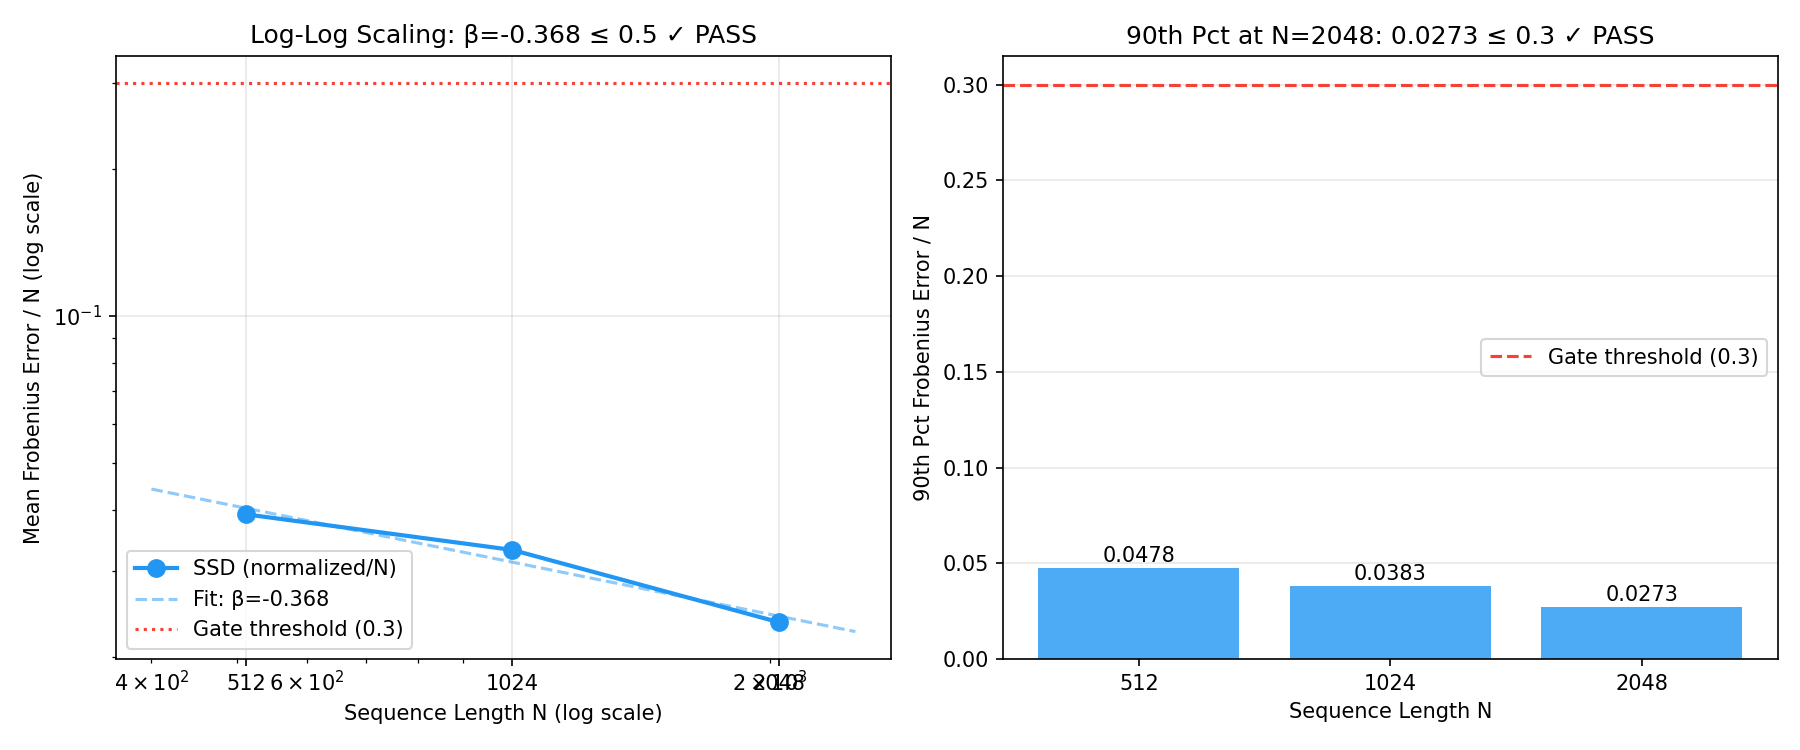
\includegraphics[width=\columnwidth]{figures/fig1_gate_bar_loglog.png}
\caption{Log-log scaling of normalized SSD Frobenius error vs N with fitted regression line ($\beta = -0.368)$ and gate threshold ($\beta$ = 0.5) annotated.}
\label{fig:fig1_gate_bar_loglog}
\end{figure}

\textbf{Figure 1.} Log-log scaling of normalized SSD Frobenius error versus sequence length N, with fitted regression line ($\beta = -0.368)$ and gate threshold ($\beta$ = 0.5) annotated. 90th percentile bars are shown with the threshold (0.3).

\begin{figure}[htbp]
\centering
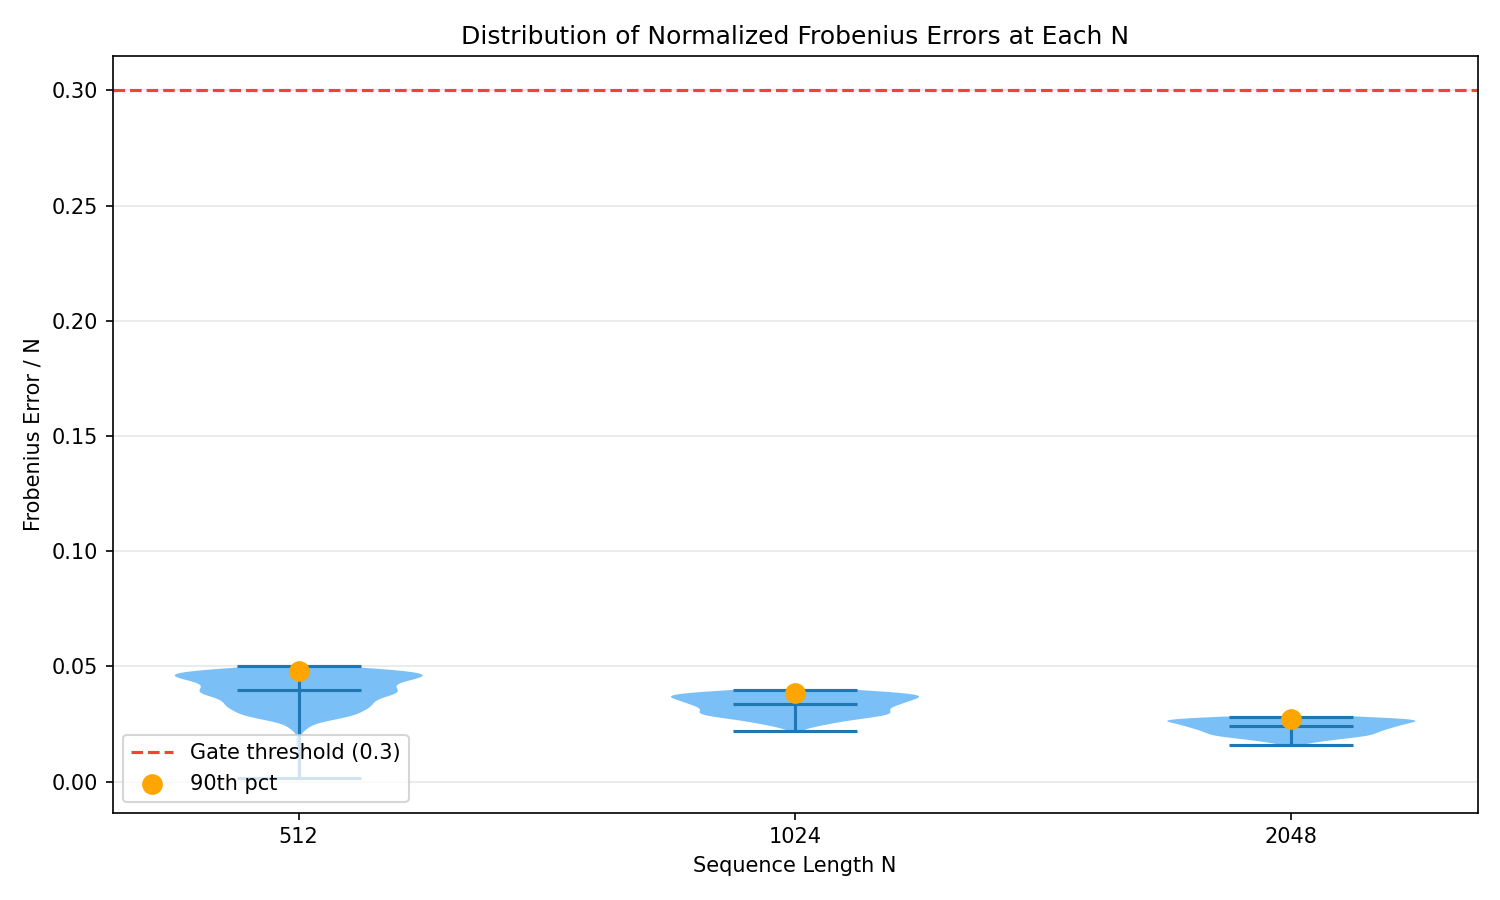
\includegraphics[width=\columnwidth]{figures/fig2_violin_distribution.png}
\caption{Violin distributions of normalized error at N $\in$ {512, 1024, 2048}.}
\label{fig:fig2_violin_distribution}
\end{figure}

\textbf{Figure 2.} Violin distributions of normalized error at N $\in$ {512, 1024, 2048} (1,600 / 160 / 160 measurements respectively). The distribution shifts downward as N increases, with no layer-level outliers.

\textbf{Interpretation:} SSD approximation quality is not the bottleneck for long-context inference in MOHAWK-converted LLaMA-3.1-8B. Any retrieval degradation observed in behavioral evaluation must be attributed to the bounded-state state update h\_t = $A\cdot h_{t-1} + B\cdot x_t$, which exponentially discounts early token positions independently of how well the SSD weights align with teacher attention matrices.

\subsubsection{5.2 Behavioral Comparison Infrastructure (RQ2, RQ3)}

All pipeline components for the behavioral comparison are validated:

\begin{itemize}
\item \textbf{Unit tests:} 22/22 passing (3.2 seconds total)
\item \textbf{Test coverage:} config validation, $\Delta _norm$ computation, bootstrap CI, mixed-effects regression, Holm correction, LongBench v2 loading, MCQ scoring, category mapping, figure generation
\item \textbf{Experiment status:} MOHAWK Stage 1 launched on $4\times$ H100 NVL GPUs (PIDs 786132--786135, Stage 1 active at report time). Stages 2 and 3, LAWCAT phases, Hybrid-4 training, LongBench v2 evaluation, and statistical analysis are all queued sequentially.
\end{itemize}

Final $\Delta _norm$ ratio and interaction p-value are not available at the time of this report. No behavioral claims are made.

\subsubsection{5.3 Implementation Issue Resolution}

Ten previously undocumented integration failure modes were identified and resolved during pipeline development for MOHAWK + LAWCAT + LLaMA-3.1-8B:

\begin{table}[htbp]
\centering
\resizebox{\columnwidth}{!}{%
\begin{tabular}{llll}
\toprule
\# & Issue & Root cause & Resolution \\
\midrule
1 & Model ID error & `meta-llama/Llama-3-8B` does not exist on HuggingFace & Use `meta-llama/Llama-3.1-8B` \\
2 & C4 rate limit (HTTP 429) & `allenai/c4` unavailable & Use `monology/pile-uncopyrighted` \\
3 & `AutoModelForCausalLM` failure & MOHAWK uses custom SSM architecture & Use MOHAWK `lazy\_init` mode=inference \\
4 & LAWCAT dataset missing & `c4\_distill` module does not exist in LAWCAT repo & Use `alpaca\_clean` native loader \\
5 & `norm\_epsilon` attribute & `LlamaBlock.py` lacks the attribute & `getattr(..., 'norm\_epsilon', 1e-5)` \\
6 & `allow\_unexpected\_keys` & `lm\_head.weight` flagged (tied-embeddings model) & Set `allow\_unexpected\_keys: true` \\
7 & `torchrun` path & Broken PATH in `youra` conda env & Use `Path(sys.executable).parent / ''torchrun''` \\
8 & Data loader chain & Missing HFDataset $\rightarrow$ Tokenize $\rightarrow$ Packing & Implemented full chain \\
9 & Port conflict & Stale `torchrun` process on port 29501 & Use `--master\_port 29502` \\
10 & Hybrid-4 architecture & MOHAWK hybrid API incompatibility & Rewrote using `LayeredMambaLM` \\
\bottomrule
\end{tabular}
}
\end{table}

